%!TEX root = ../main.tex
\chapter{Scientific Computing with SciPy}
\label{ch:scipy}

\begin{intuition}
NumPy provides the building blocks (arrays, elementary linear algebra),
but scientists often need more specialized tools: fitting a curve
to experimental data, integrating a function, solving a system
of equations, or performing statistical tests. This is exactly the role of
\textbf{SciPy}\index{SciPy}, a library built on top of NumPy.
\end{intuition}

% ----------------------------------------------------------------
\section{Overview of SciPy}

\begin{definition}[SciPy]
\textbf{SciPy} (Scientific Python) is an open-source library that provides
efficient numerical algorithms organized into thematic submodules.
\end{definition}

\begin{center}
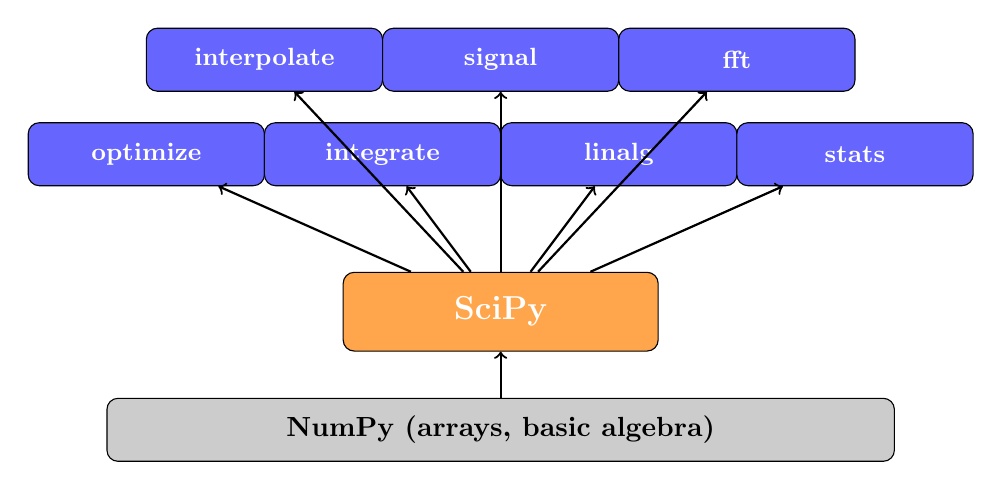
\begin{tikzpicture}[
  modbox/.style={draw, rounded corners, minimum width=3cm, minimum height=0.8cm,
                 fill=blue!60, text=white, font=\small\bfseries, align=center},
  corenode/.style={draw, rounded corners, minimum width=4cm, minimum height=1cm,
                   fill=orange!70, text=white, font=\large\bfseries, align=center},
  basenode/.style={draw, rounded corners, minimum width=10cm, minimum height=0.8cm,
                   fill=gray!40, font=\bfseries, align=center},
]
  % Base
  \node[basenode] (numpy) at (0,-3.5) {NumPy (arrays, basic algebra)};

  % Core
  \node[corenode] (scipy) at (0,-2) {SciPy};

  % Modules
  \node[modbox] (opt) at (-4.5, 0) {optimize};
  \node[modbox] (int) at (-1.5, 0) {integrate};
  \node[modbox] (lin) at (1.5, 0)  {linalg};
  \node[modbox] (sta) at (4.5, 0)  {stats};
  \node[modbox] (interp) at (-3, 1.2) {interpolate};
  \node[modbox] (sig) at (0, 1.2)  {signal};
  \node[modbox] (fft) at (3, 1.2)  {fft};

  % Arrows
  \foreach \m in {opt, int, lin, sta, interp, sig, fft}
    \draw[->, thick] (scipy) -- (\m);
  \draw[->, thick] (numpy) -- (scipy);
\end{tikzpicture}
\end{center}

% ----------------------------------------------------------------
\section{\py{scipy.optimize} --- Optimization and fitting}
\index{scipy.optimize}\index{curve\_fit}\index{minimize}

\subsection{Fitting an experimental curve with \py{curve\_fit}}

In physics, one often measures an exponential decay (radioactivity,
capacitor discharge). Let us fit a model $A(t) = A_0 \, e^{-\lambda t}$
to noisy data.

\begin{codeblock}[title=\textbf{Python}]
\begin{minted}{python}
import numpy as np
from scipy.optimize import curve_fit
import matplotlib.pyplot as plt

# Exponential model
def decay(t, A0, lam):
    return A0 * np.exp(-lam * t)

# Simulated data (with noise)
np.random.seed(42)
t_data = np.linspace(0, 10, 20)
y_data = 5.0 * np.exp(-0.3 * t_data) + 0.2 * np.random.randn(20)

# Fitting
popt, pcov = curve_fit(decay, t_data, y_data)
A0_fit, lam_fit = popt
print(f"A0 = {A0_fit:.3f}, lambda = {lam_fit:.3f}")
\end{minted}
\end{codeblock}

\begin{codeoutput}
\begin{verbatim}
A0 = 5.047, lambda = 0.308
\end{verbatim}
\end{codeoutput}

The recovered values ($A_0 \approx 5.05$, $\lambda \approx 0.31$) are close
to the true parameters ($A_0 = 5$, $\lambda = 0.3$).

\begin{codeblock}[title=\textbf{Python}]
\begin{minted}{python}
# Visualization
t_fine = np.linspace(0, 10, 200)
plt.scatter(t_data, y_data, label="Data", color="black", s=20)
plt.plot(t_fine, decay(t_fine, *popt), "r-", label="Fit")
plt.xlabel("Time (s)")
plt.ylabel("Activity (Bq)")
plt.title("Exponential decay fit")
plt.legend()
plt.show()
\end{minted}
\end{codeblock}

\subsection{Minimization with \py{minimize}}

\begin{codeblock}[title=\textbf{Python}]
\begin{minted}{python}
from scipy.optimize import minimize

# Find the minimum of f(x) = (x - 3)^2 + 2*sin(x)
def f(x):
    return (x - 3)**2 + 2 * np.sin(x)

result = minimize(f, x0=0)  # Starting point x0 = 0
print(f"Minimum at x = {result.x[0]:.4f}")
print(f"Value f(x) = {result.fun:.4f}")
\end{minted}
\end{codeblock}

\begin{codeoutput}
\begin{verbatim}
Minimum at x = 3.3424
Value f(x) = -1.8770
\end{verbatim}
\end{codeoutput}

% ----------------------------------------------------------------
\section{\py{scipy.integrate} --- Numerical integration}
\index{scipy.integrate}\index{quad}

The function \py{quad}\index{quad} computes a definite integral numerically.

\begin{definition}[Numerical integration]
Numerical integration (or quadrature) approximates the value of a definite
integral $\int_a^b f(x)\,dx$ by evaluating $f$ at a finite number of points.
\end{definition}

\begin{codeblock}[title=\textbf{Python}]
\begin{minted}{python}
from scipy.integrate import quad

# Compute the integral of sin(x) from 0 to pi
result, error = quad(np.sin, 0, np.pi)
print(f"Integral of sin(x) from 0 to pi = {result:.6f}")
print(f"Exact value = {2.0:.6f}")

# Gaussian integral: int from -inf to +inf of exp(-x^2)
val, err = quad(lambda x: np.exp(-x**2), -np.inf, np.inf)
print(f"Gaussian integral = {val:.6f}")
print(f"sqrt(pi) = {np.sqrt(np.pi):.6f}")
\end{minted}
\end{codeblock}

\begin{codeoutput}
\begin{verbatim}
Integral of sin(x) from 0 to pi = 2.000000
Exact value = 2.000000
Gaussian integral = 1.772454
sqrt(pi) = 1.772454
\end{verbatim}
\end{codeoutput}

% ----------------------------------------------------------------
\section{\py{scipy.linalg} --- Linear algebra}
\index{scipy.linalg}\index{solve}\index{eig}

\subsection{Solving a linear system}

Consider the system:
\[
\begin{cases}
2x + y = 5 \\
x + 3y = 7
\end{cases}
\quad \Longleftrightarrow \quad
\begin{pmatrix} 2 & 1 \\ 1 & 3 \end{pmatrix}
\begin{pmatrix} x \\ y \end{pmatrix}
=
\begin{pmatrix} 5 \\ 7 \end{pmatrix}
\]

\begin{codeblock}[title=\textbf{Python}]
\begin{minted}{python}
from scipy.linalg import solve, eig

A = np.array([[2, 1],
              [1, 3]])
b = np.array([5, 7])

x = solve(A, b)
print(f"Solution: x = {x[0]:.2f}, y = {x[1]:.2f}")
\end{minted}
\end{codeblock}

\begin{codeoutput}
\begin{verbatim}
Solution: x = 1.60, y = 1.80
\end{verbatim}
\end{codeoutput}

\subsection{Eigenvalues}

\begin{codeblock}[title=\textbf{Python}]
\begin{minted}{python}
# Eigenvalues and eigenvectors
eigenvalues, eigenvectors = eig(A)
print("Eigenvalues:", eigenvalues.real)
print("Eigenvector 1:", eigenvectors[:, 0].real)
\end{minted}
\end{codeblock}

\begin{codeoutput}
\begin{verbatim}
Eigenvalues: [1.38196601 3.61803399]
Eigenvector 1: [-0.85065081  0.52573111]
\end{verbatim}
\end{codeoutput}

% ----------------------------------------------------------------
\section{\py{scipy.stats} --- Statistics}
\index{scipy.stats}

\begin{codeblock}[title=\textbf{Python}]
\begin{minted}{python}
from scipy import stats

# Generate data following a normal distribution
np.random.seed(0)
sample = stats.norm.rvs(loc=170, scale=10, size=100)

# Descriptive statistics
print(f"Mean: {np.mean(sample):.2f}")
print(f"Std. dev.: {np.std(sample, ddof=1):.2f}")

# Normality test (Shapiro-Wilk)
stat, p = stats.shapiro(sample)
print(f"Shapiro-Wilk test: p = {p:.4f}")
if p > 0.05:
    print("-> Distribution consistent with normality")
\end{minted}
\end{codeblock}

\begin{codeoutput}
\begin{verbatim}
Mean: 171.77
Std. dev.: 10.14
Shapiro-Wilk test: p = 0.8453
-> Distribution consistent with normality
\end{verbatim}
\end{codeoutput}

\begin{codeblock}[title=\textbf{Python}]
\begin{minted}{python}
# Student's t-test (two samples)
group_a = stats.norm.rvs(loc=170, scale=10, size=50, random_state=1)
group_b = stats.norm.rvs(loc=175, scale=10, size=50, random_state=2)

t_stat, p_val = stats.ttest_ind(group_a, group_b)
print(f"t = {t_stat:.3f}, p-value = {p_val:.4f}")
\end{minted}
\end{codeblock}

\begin{codeoutput}
\begin{verbatim}
t = -2.574, p-value = 0.0116
\end{verbatim}
\end{codeoutput}

% ----------------------------------------------------------------
\section{\py{scipy.interpolate} --- Interpolation}
\index{scipy.interpolate}\index{interp1d}

Interpolation allows estimating values between measurement points.

\begin{codeblock}[title=\textbf{Python}]
\begin{minted}{python}
from scipy.interpolate import interp1d

# Measurement points (temperature as a function of time)
time = np.array([0, 1, 2, 3, 4, 5])
temperature = np.array([20.0, 22.5, 28.3, 31.1, 29.0, 25.5])

# Linear and cubic interpolation
f_lin = interp1d(time, temperature, kind="linear")
f_cub = interp1d(time, temperature, kind="cubic")

t_fine = np.linspace(0, 5, 100)
print(f"T at t=2.5 (linear): {f_lin(2.5):.2f} deg C")
print(f"T at t=2.5 (cubic):  {f_cub(2.5):.2f} deg C")
\end{minted}
\end{codeblock}

\begin{codeoutput}
\begin{verbatim}
T at t=2.5 (linear): 29.70 deg C
T at t=2.5 (cubic):  30.22 deg C
\end{verbatim}
\end{codeoutput}

\begin{codeblock}[title=\textbf{Python}]
\begin{minted}{python}
plt.scatter(time, temperature, color="black", zorder=5,
            label="Measurements")
plt.plot(t_fine, f_lin(t_fine), "--", label="Linear")
plt.plot(t_fine, f_cub(t_fine), "-", label="Cubic")
plt.xlabel("Time (h)")
plt.ylabel("Temperature (deg C)")
plt.legend()
plt.title("Temperature data interpolation")
plt.show()
\end{minted}
\end{codeblock}

% ----------------------------------------------------------------
\begin{errmark}{Common errors with SciPy}
\begin{enumerate}
  \item \textbf{Confusing \py{numpy.linalg} and \py{scipy.linalg}} ---
    Both exist, but \py{scipy.linalg} is more complete and more optimized.
    Always prefer \py{scipy.linalg} for serious computations.
  \item \textbf{Forgetting the starting point in \py{minimize}} ---
    The function \py{minimize} requires an \py{x0}. A poor initial choice can
    lead to a \emph{local} minimum instead of the global minimum.
  \item \textbf{Wrong model in \py{curve\_fit}} --- If the mathematical model
    does not match the data, the fit will be poor. Always check
    the result visually.
  \item \textbf{Ignoring the covariance matrix} --- \py{curve\_fit} also returns
    \py{pcov}, which allows computing the uncertainties on the fitted
    parameters: \py{np.sqrt(np.diag(pcov))}.
\end{enumerate}
\end{errmark}

% ----------------------------------------------------------------
\begin{projet}{Experimental data analysis and fitting}
Simulate a capacitor discharge experiment:
\begin{enumerate}
  \item Generate noisy data following $V(t) = V_0 \, e^{-t/\tau}$
    with $V_0 = 12$\,V and $\tau = 3$\,s (add Gaussian noise).
  \item Use \py{curve\_fit} to recover $V_0$ and $\tau$.
  \item Compute the uncertainties from the covariance matrix.
  \item Numerically integrate the dissipated energy:
    $E = \int_0^{20} \frac{V(t)^2}{R}\,dt$ with $R = 1\,\text{k}\Omega$.
  \item Plot the data, the fitted curve, and the error bars.
  \item Compare the obtained $\tau$ with the theoretical value.
\end{enumerate}
\end{projet}

% ----------------------------------------------------------------
\section{Exercises}

\begin{exercise}[$\star$]
Numerically compute the integral $\displaystyle\int_0^1 e^{-x^2}\,dx$ with
\py{quad}. Compare with the approximate value $\approx 0.7468$.
\end{exercise}

\begin{exercise}[$\star$]
Solve the linear system:
$3x + 2y - z = 1$, $2x - y + 4z = -2$, $x + y + z = 0$.
Verify by computing $A \cdot x$ with NumPy.
\end{exercise}

\begin{exercise}[$\star\star$]
Generate 200 points following a normal distribution ($\mu = 50$, $\sigma = 8$).
Perform a Shapiro-Wilk test and a Kolmogorov-Smirnov test
(\py{stats.kstest}) to check for normality. Interpret the p-values.
\end{exercise}

\begin{exercise}[$\star\star$]
Experimental data follow the law $y = a \sin(bx + c)$.
Generate data with $a=3$, $b=2$, $c=0.5$ plus noise.
Use \py{curve\_fit} to recover the parameters. Note: provide
reasonable initial values with the \py{p0} parameter.
\end{exercise}

\begin{exercise}[$\star\star\star$]
Model the kinetics of a second-order chemical reaction:
$\frac{d[A]}{dt} = -k[A]^2$. The analytical solution is
$[A](t) = \frac{[A]_0}{1 + k[A]_0 t}$. Generate noisy data,
fit the model to find $k$ and $[A]_0$, then numerically integrate
$\int_0^{10} [A](t)\,dt$ (total remaining quantity). Compare numerical
integration with the analytical solution.
\end{exercise}

% ----------------------------------------------------------------
\begin{keyformulas}{Chapter 10 --- SciPy: the essentials}
\begin{tabular}{@{}p{4.5cm} p{9.5cm}@{}}
\toprule
\textbf{Submodule} & \textbf{Key functions} \\
\midrule
\py{scipy.optimize} & \py{minimize(f, x0)}, \py{curve\_fit(model, x, y)} \\
\py{scipy.integrate} & \py{quad(f, a, b)} --- definite integral \\
\py{scipy.linalg} & \py{solve(A, b)}, \py{eig(A)} \\
\py{scipy.stats} & \py{ttest\_ind}, \py{shapiro}, distributions \\
\py{scipy.interpolate} & \py{interp1d(x, y, kind="cubic")} \\
\midrule
\multicolumn{2}{@{}l}{\textbf{Tips}} \\
\midrule
Fit uncertainties & \py{np.sqrt(np.diag(pcov))} \\
Infinite bounds & \py{quad(f, -np.inf, np.inf)} \\
Initial values & \py{curve\_fit(f, x, y, p0=[a0, b0])} \\
\bottomrule
\end{tabular}
\end{keyformulas}
